\chapter{Multi-Group Cross-Section Generation}
\label{chap:mgxs}

In the previous chapter, the neutron transport equation was derived from fundamentals. The final form presented at the end of the chapter relied on the availability of accurate multi-group cross-sections. However, these quantities rely on scalar and angular fluxes, which require the solution of the neutron transport equation. In this chapter, the nature of continuous energy cross-sections are discussed in Section~\ref{sec:continuous-energy-xs}. Then the application of continuous energy Monte Carlo methods is introduced in Section~\ref{sec:monte-carlo}. The addition of tallies to Monte Carlo is introduced in Section~\ref{sec:mc-tallies}. The application of Monte Carlo methods to form estimates of multi-group cross-sections is discussed in Section~\ref{sec:mc-xs-generation}. For most deterministic codes, including OpenMOC, the angular dependence of total cross-sections is ignored. The implications of this are discussed in Section~\ref{sec:mgxs-angular-dependence}. Then, the transport correction is discussed in Section~\ref{sec:transport-correction}. Finally, Section~\ref{sec:mgxs-implications} discusses the practical implications of multi-group cross-section generation.

\section{Continuous Energy Cross-Sections}
\label{sec:continuous-energy-xs}

Recall from Chapter~\ref{chap:transport} that the macroscopic cross-sections appearing in the neutron transport equation in Eq.~\ref{eqn:full-multi-group-transport} are formed by the product of isotopic microscopic cross-sections and number density. Microscopic cross-sections are intensive properties of the isotopes comprising the material whereas number density can be directly calculated with material density and material composition. The macroscopic cross-section can be thought of as a linear combination of the microscopic cross-sections of the material's comprising isotopes. The shape of macroscopic cross-sections in energy are therefore determined by the shape of microscopic cross-sections.

Since microscopic cross-sections are intensive isotopic properties, they can be experimentally measured in a laboratory. These cross-sections are dependent on the relative motion of the impingent neutron and the target nuclei. Therefore thermal motion of target causes cross-sections to be temperature dependent. The energy dependence of microscopic cross-section can be quite complicated. Microscopic cross-sections typically have many \textit{resonance} energies~\cite{compound-nucleus, bell1970nuclear} at which the cross-section varies by orders of magnitude. An example of typical cross-section energy dependence is shown in Figure~\ref{fig:microscopic-xs}.
\begin{figure}[h!]
	\centering
	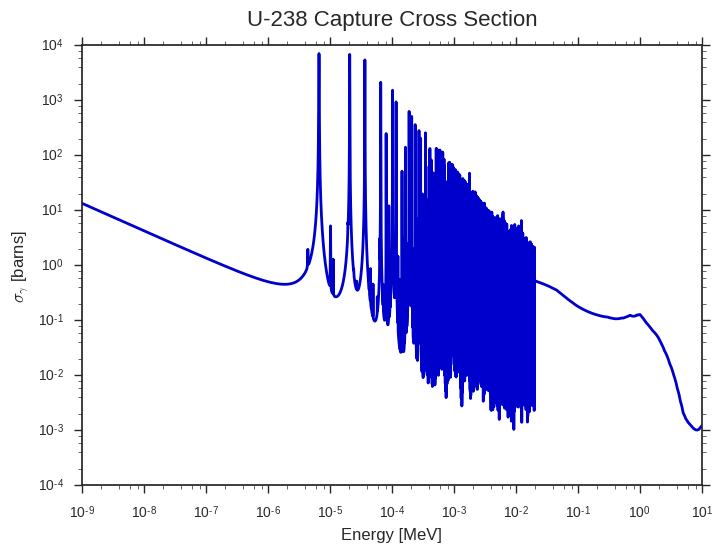
\includegraphics[width=0.9\linewidth]{figures/u238-capture-xs.png}
	\caption[]{The microscopic capture cross-section of U-238.}
	\label{fig:microscopic-xs}
\end{figure}

The challenge of forming multi-group cross-sections is to transform this intricate energy dependence into energy ranges over which the behavior can be sufficiently captured by a constant value. A depiction of this challenge is shown in Figure~\ref{fig:microscopic-to-multigroup}. While the task of capturing the energy behavior in this manner might seem unachievable, appropriate weighting with the neutron flux can reduce the approximation error while greatly reducing the computational complexity of modeling the neutron behavior.
\begin{figure}[h!]
	\centering
	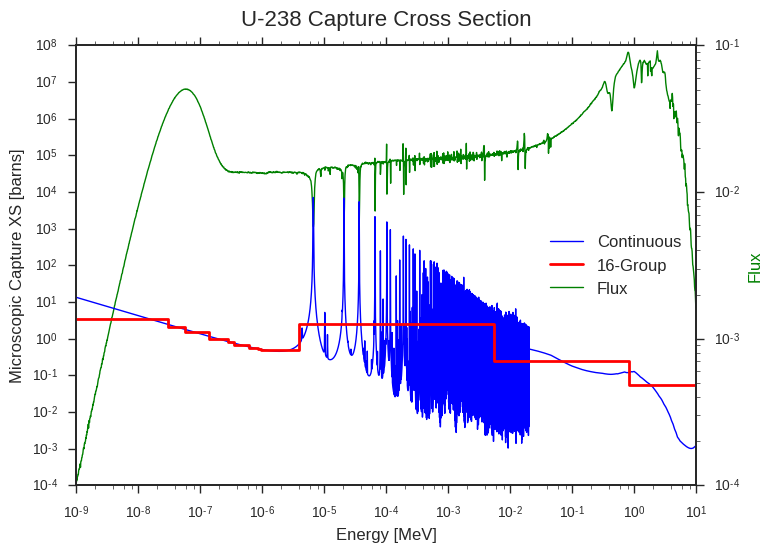
\includegraphics[width=0.9\linewidth]{figures/u238-capture-16.png}
	\caption[]{An illustration of forming multi-group cross-sections from continuous energy cross-sections showing the continuous energy capture cross-section of U-238 (blue), the neutron flux (green), and the multi-group representation with 16 groups (red).}
	\label{fig:microscopic-to-multigroup}
\end{figure}

\section{Analog Continuous Energy Monte Carlo Simulation}
\label{sec:monte-carlo}

Monte Carlo is a popular technique to solve for neutron behavior since it incorporates very few approximations and assumptions. Popular Monte Carlo codes include MCNP\cite{mcnpx2003manual}, Serpent\cite{leppanen2007serpent}, and OpenMC\cite{romano2013openmc}, as well as many others. This section briefly describes Monte Carlo simulation. The interested reader is encouraged to explore the OpenMC user manual\cite{openmc2016manual} for a more complete description of Monte Carlo methods.

Directly from the continuous energy cross-section data discussed in the previous section, Monte Carlo solvers can solve the transport equation for the neutron flux and reaction rates. Rather than explicitly solving the partial differential equation form of the neutron transport equation, Monte Carlo treats neutron behavior as a stochastic process characterized by underlying probability distributions.

This is done by simulating individual neutron histories describing a neutron's behavior from its creation to its absorption or leakage. The reactor behavior is determined by the average of many neutron histories. Each history is determined by sampling the underlying probability distributions, often characterized by the continuous energy cross-section data.

At the beginning of a neutron history, the neutron location $\mathbf{r}$, direction $\mathbf{\Omega}$, and energy $E$ are sampled from the source distribution emitting the neutron, such as fission. For a fission source, the location $\mathbf{r}$ is sampled from the fission rate distribution. The initial direction $\mathbf{\Omega}$ is usually assumed to be isotropic, and the energy is sampled from the fission emission spectrum $\chi$. 

Once the direction and energy are sampled, the distance to collision is sampled from an exponential distribution with mean distance to collision $1/\Sigma_{t}(\mathbf{r},E)$. Therefore the distance $d$ can be sampled by computing
\begin{equation}
d = \frac{-\ln{\epsilon}}{\Sigma_{t}(\mathbf{r},E)}
\end{equation}
where $\epsilon$ is a uniformly distributed random variable between 0 and 1, whose sampling is commonly available to most software languages. Once the distance is sampled, the neutron is moved in the direction of travel. If the neutron leaves the geometry boundaries, its history ends and ceases to be tracked.

If the neutron's new position is within geometry boundaries, it interacts at the collision point. The type of interaction can either be scattering or absorption. Since cross-sections are related to interaction probability, the probability of absorption $p_a$ can be computed as
\begin{equation}
	p_a = \Sigma_a(\mathbf{r},E) / \Sigma_{t}(\mathbf{r},E)
\end{equation}
where $\Sigma_a(\mathbf{r},E)$ is the absorption cross-section. The scattering probability is then $1-p_a$. Therefore, absorption occurs if a newly sampled uniform variable $\epsilon$ is less than $p_a$.

During absorption events, the type of absorption is simulated in a very similar way. The two types of absorption events are capture and fission, each with a defined cross-section. The ratio of cross-sections to the absorption cross-section yields the associated probabilities. During neutron capture events, the neutron is simply absorbed by target nuclei without releasing additional neutrons. During fission events, the neutron is again absorbed, but the number of neutrons released from fission is sampled. The location of interaction and number of neutrons released is noted and added to a fission bank, which may be used as a fission source site for the starting location of other neutron histories.

During scattering events, the neutron's behavior is treated directly with scattering mechanics. In the center of momentum frame, neutrons scatter isotropically during elastic scattering events. Therefore, the neutron's trajectory is transformed to the center of momentum frame where a new scattering direction and energy are sampled. Then the neutron's trajectory is transformed back to the laboratory frame. This allows the scattering to be treated explicitly without the need for significant approximation. After scattering, a new distance to collision is sampled and the process is continued until the neutron eventually leaks or is absorbed. 


The Monte Carlo description described here is the analog form of Monte Carlo. However, in practice, many variance reduction techniques are used to improve Monte Carlo efficiency without injecting any bias so that the mean is preserved. These techniques, while mathematically sound, obscure the treatment of neutron behavior as it explicitly exists in nature. Therefore, while the analog description was chosen here to demonstrate the principles of Monte Carlo, any reasonable Monte Carlo implementation would incorporate many variance reduction techniques.

\section{Monte Carlo Tallies}
\label{sec:mc-tallies}

The Monte Carlo process described in the previous section would run, faithfully follow neutrons according to the underlying physics, but yield no tangible results. In order to obtain useful results, quantities need to be recorded during the simulation of each neutron. These records are termed \textit{tallies} which usually record average neutron behavior.

Since Monte Carlo directly simulates neutron behavior, it can directly tally reaction rates. For instance, Monte Carlo simulations can directly tally the probability that source neutrons induce fission in a given region by simply recording the number of neutrons that induce fission and dividing that tally by the total number of source neutrons. Scaling this probability with the neutron source strength directly yields the fission rate in the region. This procedure can be used to compute the rate of any reaction simulated in the Monte Carlo implementation.

In addition to calculating reaction rates, the neutron scalar flux can also be computed. There are two main ways of tallying the scalar flux: the collision estimator and the track length estimator. The collision estimator calculates the flux that would induce an observed collision rate. The track length estimator is a variation reduction technique which is capable of tallying a contribution to the local scalar flux even when no collision occurs.

\section{Monte Carlo Generation of Multi-Group Cross-Sections}
\label{sec:mc-xs-generation}

The two quantities that need to be computed in order to form multi-group cross-sections are reaction rates and scalar fluxes. For instance the multi-group fission cross-section $\Sigma_f^g\left(\mathbf{r}\right)$ for energy group $g$ is computed as
\begin{equation}
\Sigma_f^g\left(\mathbf{r}\right) = \frac{\int\displaylimits_{E_{g'-1}}^{E_{g'}} dE \, \Sigma_f(\mathbf{r}, E) \phi(\mathbf{r}, E)}{\int\displaylimits_{E_{g'-1}}^{E_{g'}} dE \, \phi(\mathbf{r}, E)} 
\end{equation}
where the numerator represents a reaction rate and the denominator is the scalar flux, both integrated over the energy group width.

There is a long history of using approximations to the scalar flux to compute multi-group cross-sections~\cite{cacuci2010handbook}. However, since reaction rates and scalar fluxes can both be tallied directly in Monte Carlo, there is no need for such approximations with direct Monte Carlo simulation. The downside of this approach is the potentially large computational required to compute cross-sections in every zone of interest. One of the earliest known in-depth analysis of multi-group cross-section generation using Monte Carlo was performed by Redmond~\cite{redmond1997multigroup} studying computation of group-to-group scattering moment matrices in the MCNP code~\cite{mcnpx2003manual}. This work was further expanded by Fridman~\cite{fridman2011serpent} with the Serpent code for few group cross-section generation intended for diffusion solvers.

Recently, Boyd leveraged increases in computation power and machine learning to efficiently compute accurate multi-group cross-sections~\cite{boyd2017thesis}. Boyd applied his multi-group cross-sections to multi-group transport solvers rather than standard diffusion solvers. The machine learning tools analyzed patterns within the Monte Carlo simulation data to determine regions with similar cross-sections. By identifying these regions, the Monte Carlo statistics can be averaged over all similar regions, allowing for quicker convergence. 

While his focus proved that machine learning tools could be implemented to form accurate multi-group cross-sections, the work also showed that if many energy groups are requested (more than $\approx50$), the spatial variation in cross-sections was very small. This allows cross-sections to be formed for unique materials rather than unique regions, if a large number of energy groups are allowed. Since there are many more unique regions than unique materials, this greatly simplifies the cross-section generation process. The work in this thesis concentrates on using a high number of energy groups so the spatial sensitivity of cross-sections is small. However, a move to fewer number of energy groups would allow the deterministic methods using the multi-group cross-sections to be far more efficient.


\section{Angular Dependence of Total Cross-Sections}
\label{sec:mgxs-angular-dependence}

From the definition of the multi-group total cross section in Eq.~\ref{eqn:multi-group-xs-definitions-first}, 
\begin{equation*}
	\Sigma_{t}^g(\mathbf{r},\mathbf{\Omega}) = \frac{\int_{E_{g-1}}^{E_g} dE \, \Sigma_{t}(\mathbf{r},E)\psi(\mathbf{r},\mathbf{\Omega},E)}{\int_{E_{g-1}}^{E_g} dE \, \psi(\mathbf{r},\mathbf{\Omega},E)} ,
\end{equation*}
it is clear that the multi-group total cross-section should be angular dependent even though we assume the continuous energy total cross-section is angular independent. This is because the total cross-section multiplies the angular flux rather than the scalar flux. In turn, this causes its collapsed multi-group form to be angular dependent since both the numerator and denominator of the expression in Eq.~\ref{eqn:multi-group-xs-definitions-first} are angular dependent. This would be true of any cross-section that multiplies the angular flux, but with the isotropic scattering approximation, there are no other terms that multiply cross-sections by the angular flux.

This angular dependence is often neglected, but can introduce a bias~\cite{gibson-preprint}. With the angular dependence ignored, the relationship can be integrated over all directions leading to the form in Eq.~\ref{eqn:tot-mgxs-sf}.
\begin{equation}
\Sigma_{t}^g(\mathbf{r}) = \frac{\int_{E_{g-1}}^{E_g} dE \, \Sigma_{t}(\mathbf{r},E)\phi(\mathbf{r},E)}{\int_{E_{g-1}}^{E_g} dE \, \phi(\mathbf{r},E)} 
\label{eqn:tot-mgxs-sf}
\end{equation}
The work in this thesis also relies on the approximation of angular independent multi-group total cross-sections. With this approximation, the new multi-group transport equation is given in Eq.~\ref{eqn:multi-group-transport}. The solution of this equation is the subject of this thesis. 
\begin{equation}
\mathbf{\Omega} \cdot \nabla \psi_{g}(\mathbf{r},\mathbf{\Omega}) + \Sigma_t^{g}(\mathbf{r}) \psi_{g}(\mathbf{r},\mathbf{\Omega}) = \frac{1}{4 \pi} \left( \frac{\chi_{g}\left(\mathbf{r}\right)}{k} \sum_{g'=1}^{G} \nu_{g'}\left(\mathbf{r}\right) \Sigma_f^{g'}\left(\mathbf{r}\right) \phi_{g'}\left(\mathbf{r}\right) + \, \sum_{g'=1}^G \,  \Sigma_{s}^{g' \rightarrow g}\left(\mathbf{r}\right) \phi_{g'}(\mathbf{r}) \right)
\label{eqn:multi-group-transport}
\end{equation}
It is important to remember that some error is expected from the absence of angular dependent total cross-sections so that the multi-group transport solution does not strictly match the corresponding continuous energy transport solution, such as that computed by Monte Carlo methods.

\section{The Transport Correction}
\label{sec:transport-correction}

Previously it was mentioned that the assumption of isotropic scattering introduces significant bias, but is remedied by a transport correction. In this section, the transport correction is derived and its implications are discussed. Many different transport corrections have been implemented, such as those described in the TRANSX~\cite{macfarlane1993transx} and NJOY~\cite{macfarlane2000njoy} manuals. The basis for these transport corrections was formulated by Bell, Hansen and Sandmeier~\cite{bell1967transport}. However, this section largely follows Hebert's derivation~\cite{hebert2009applied}. 

Recall from Eq.~\ref{eqn:xs-angular-dependence-removal} that the scattering term, without the isotropic assumption, follows the relationship
\begin{equation*}
\int\displaylimits_{0}^{\infty} dE' \, \int\displaylimits_{4\pi} \, d\mathbf{\Omega'} \Sigma_{s}(\mathbf{r}, \mathbf{\Omega'}\rightarrow \mathbf{\Omega},{E'\rightarrow E}) \psi(\mathbf{r}, \mathbf{\Omega'},E').
\end{equation*}
In the laboratory system, in which neutron behavior is modeled, scattering may be strongly anisotropic. However, in the center-of-momentum framework, scattering is nearly isotropic in the energy range of interest. This implies that the angular dependence relies on the magnitude of the deflection from scattering $\mathbf{\Omega} \cdot \mathbf{\Omega'}$, reducing this relationship to
\begin{equation*}
	\int\displaylimits_{0}^{\infty} dE' \, \int\displaylimits_{4\pi} \, d\mathbf{\Omega'} \Sigma_{s}(\mathbf{r}, \mathbf{\Omega} \cdot \mathbf{\Omega'},{E'\rightarrow E}) \psi(\mathbf{r}, \mathbf{\Omega'},E').
\end{equation*}
The scattering kernel can be expressed as an expansion of Legendre polynomials $P_\ell$ with angular-independent coefficients $\Sigma_{s,\ell}\left(\mathbf{r}, E'\rightarrow E \right)$ as shown in Eq.~\ref{eqn:scattering-expansion} where $\mu = \mathbf{\Omega} \cdot \mathbf{\Omega'}$.
\begin{equation}
 \Sigma_{s}(\mathbf{r}, \mu,{E'\rightarrow E}) = \sum_{\ell=0}^\infty \frac{2 \ell + 1}{2} \Sigma_{s,\ell}\left(\mathbf{r}, E'\rightarrow E \right) P_\ell(\mu)
 \label{eqn:scattering-expansion}
\end{equation}
The coefficients can be determined by taking advantage of the orthogonality of Legendre polynomials, leading to the relationship in Eq.~\ref{eqn:scattering-expansion-coefficients}.
\begin{equation}
\Sigma_{s,\ell}\left(\mathbf{r}, E'\rightarrow E \right) = \int_{-1}^{1} d\mu \, \Sigma_{s}(\mathbf{r}, \mu, {E'\rightarrow E}) P_\ell(\mu)
\label{eqn:scattering-expansion-coefficients}
\end{equation}
The scattering kernel can be approximated by a finite number $L$ of Legendre polynomials with modified coefficients $\tilde{\Sigma}_{s,\ell}\left(\mathbf{r}, E'\rightarrow E \right)$ and a transport correction term $\Delta \Sigma_{\textit{tr}}\left(\mathbf{r}, E'\rightarrow E \right)$ in Eq.~\ref{eqn:scattering-expansion-approx}.
\begin{equation}
\Sigma_{s}(\mathbf{r}, \mu, {E'\rightarrow E}) \approx \sum_{\ell=0}^L \frac{2 \ell + 1}{2} \tilde{\Sigma}_{s,\ell}\left(\mathbf{r}, E'\rightarrow E \right) P_\ell(\mu) + \Delta \Sigma_{\textit{tr}}\left(\mathbf{r}, E'\rightarrow E \right) \delta\left(\mu - 1\right)
\label{eqn:scattering-expansion-approx}
\end{equation}
Here $\delta$ represents the Dirac delta function, whose application to the transport correction makes the term forward peaked in the direction of travel to capture higher order anisotropies. Taking advantage of the relationship in Eq.~\ref{eqn:scattering-expansion-coefficients} and the approximation of the scattering kernel in Eq.~\ref{eqn:scattering-expansion-approx}, the true Legendre polynomial scattering coefficients can be related to the modified coefficients in Eq.~\ref{eqn:scattering-expansion-coefficients-approx}
\begin{equation}
\begin{split}
\Sigma_{s,\ell}\left(\mathbf{r}, E'\rightarrow E \right) \approx \int_{-1}^{1} d\mu \, \sum_{\ell'=0}^L \frac{2 \ell' + 1}{2} \tilde{\Sigma}_{s,\ell'}\left(\mathbf{r}, E'\rightarrow E \right) P_{\ell'}(\mu) P_\ell(\mu) \\ + \int_{-1}^{1} d\mu \, \Delta \Sigma_{\textit{tr}}\left(\mathbf{r}, E'\rightarrow E \right) \delta\left(\mu - 1\right) P_\ell(\mu)
\label{eqn:scattering-expansion-coefficients-approx}
\end{split}
\end{equation}
For $0 \leq \ell \leq L$, Eq.~\ref{eqn:scattering-expansion-coefficients-approx} can be simplified using the orthogonality of Legendre polynomials and the property $P_\ell(1) = 1$. This leads to the simplified relationship in Eq.~\ref{eqn:tc-simplified-coefficients}.
\begin{equation}
\Sigma_{s,\ell}\left(\mathbf{r}, E'\rightarrow E \right) \approx  \tilde{\Sigma}_{s,\ell}\left(\mathbf{r}, E'\rightarrow E \right) + \Delta \Sigma_{\textit{tr}}\left(\mathbf{r}, E'\rightarrow E \right)
\label{eqn:tc-simplified-coefficients}
\end{equation}
In order to capture the next order scattering after $L$, the transport correction term is set to capture scattering of order $L+1$ as shown in Eq.~\ref{eqn:tc-scattering-order}.
\begin{equation}
\Delta \Sigma_{\textit{tr}}\left(\mathbf{r}, E'\rightarrow E \right) = \Sigma_{s,L+1}\left(\mathbf{r}, E'\rightarrow E \right)
\label{eqn:tc-scattering-order}
\end{equation}
For isotropic in lab scattering with $L=0$, the scattering kernel takes the form of Eq.~\ref{eqn:tc-scattering-kernel}, following the form of Eq.~\ref{eqn:scattering-expansion-approx}, where the transport correction term compensates for first order scattering in the direction of travel.
\begin{equation}
\begin{split}
	\Sigma_{s}(\mathbf{r},\mathbf{\Omega'} \rightarrow \mathbf{\Omega},E'\rightarrow E) \approx & \frac{1}{4\pi}\left[\Sigma_{s,0}(\mathbf{r},{E'\rightarrow E}) - \Sigma_{s,1}(\mathbf{r},{E'\rightarrow E})\right] \\ & + \, \Sigma_{s,1}(\mathbf{r},{E'\rightarrow E})\delta(\mathbf{\Omega'} \cdot \mathbf{\Omega}-1)
\end{split}
\label{eqn:tc-scattering-kernel}
\end{equation}
Inserting this definition of the scattering kernel into Eq.~\ref{eqn:xs-angular-dependence-removal}, the continuous energy and angle transport equation becomes:
\begin{equation}
\begin{split}
\mathbf{\Omega} \cdot \nabla \psi(\mathbf{r},\mathbf{\Omega},E) \, + & \, \Sigma_{t}(\mathbf{r},E)\psi(\mathbf{r},\mathbf{\Omega},E) = \\
& \phantom{+} \, \frac{\chi(\mathbf{r},E)}{4\pi k} \int\displaylimits_{0}^{\infty} dE' \, \nu(\mathbf{r},E') \Sigma_f(\mathbf{r}, E') \phi(\mathbf{r}, E')\\
& + \, \int\displaylimits_{0}^{\infty} dE' \, \int\displaylimits_{4\pi} \, d\mathbf{\Omega'} \Bigg( \frac{1}{4 \pi} \left[\Sigma_{s,0}(\mathbf{r},{E'\rightarrow E}) - \Sigma_{s,1}(\mathbf{r},{E'\rightarrow E}) \right]\\
& \phantom{\frac{1}{4 \pi}\int\displaylimits_{0}^{\infty} dE' \, \int\displaylimits_{4\pi}\, d\mathbf{\Omega'}} + \, \Sigma_{s,1}(\mathbf{r},{E'\rightarrow E})\delta(\mathbf{\Omega'} \cdot \mathbf{\Omega}-1)\Bigg) \psi(\mathbf{r}, \mathbf{\Omega'},E')
\end{split}
\end{equation}
Taking advantage of the Dirac delta function in the transport correction term as well as the angular independence of the other scattering terms, this relationship can be simplified, as shown in Eq.~\ref{eqn:transport-tc-energy-dependent}.
\begin{equation}
\begin{split}
\mathbf{\Omega} \cdot \nabla \psi(\mathbf{r},\mathbf{\Omega},E) \, + & \, \Sigma_{t}(\mathbf{r},E)\psi(\mathbf{r},\mathbf{\Omega},E) - \, \int\displaylimits_{0}^{\infty} dE' \, \Sigma_{s,1}(\mathbf{r},{E'\rightarrow E}) \psi(\mathbf{r},\mathbf{\Omega}, E') = \\
& \phantom{+} \, \frac{\chi(\mathbf{r},E)}{4\pi k} \int\displaylimits_{0}^{\infty} dE' \, \nu(\mathbf{r},E') \Sigma_f(\mathbf{r}, E') \phi(\mathbf{r}, E')\\
& + \, \frac{1}{4 \pi}\int\displaylimits_{0}^{\infty} dE' \, \left( \Sigma_{s,0}(\mathbf{r},{E'\rightarrow E}) - \Sigma_{s,1}(\mathbf{r},{E'\rightarrow E}) \right) \phi(\mathbf{r}, E')
\end{split}
\label{eqn:transport-tc-energy-dependent}
\end{equation}
A transport correction independent of outgoing neutron energy is defined in Eq.~\ref{eqn:energy-indep-tc}. Similar to how the multi-group total cross-section is angle dependent, but the continuous energy total cross-section is independent of angle, the transport correction also becomes angular dependent.
\begin{dmath}
	\Delta\Sigma_{tr}(\mathbf{r}, \mathbf{\Omega}, E) = \frac{\int\displaylimits_{0}^{\infty} dE' \, \Sigma_{s,1}(\mathbf{r},{E'\rightarrow E})\psi(\mathbf{r},\mathbf{\Omega},E')}{\psi(\mathbf{r},\mathbf{\Omega},E)}
	\label{eqn:energy-indep-tc}
\end{dmath}
However, similar to how the angular dependence of the total cross-section is ignored, the angular dependence of the transport correction is also ignored. In this thesis the same approximation is invoked. Although this approximation could be significant, the use of a first order correction for the transport correction already introduces some bias. Taking the transport correction to be angular independent, the transport correction is defined in terms of scalar fluxes in Eq.~\ref{eqn:transport-correction}.
\begin{dmath}
	\Delta\Sigma_{tr}(\mathbf{r}, E) = \frac{\int\displaylimits_{0}^{\infty} dE' \, \Sigma_{s,1}(\mathbf{r},{E'\rightarrow E})\phi(\mathbf{r},E')}{\phi(\mathbf{r},E)}
	\label{eqn:transport-correction}
\end{dmath}
This leads to a transport equation that appears very similar to the isotropic form derived in Chapter~\ref{chap:transport}, as shown in Eq.~\ref{eqn:tc-transport-cont-energy}
\begin{equation}
\begin{split}
\mathbf{\Omega} \cdot \nabla \psi(\mathbf{r},\mathbf{\Omega},E) \, + & \, \Sigma_{\textit{tr}}(\mathbf{r},E)\psi(\mathbf{r},\mathbf{\Omega},E) = \\
\frac{\chi(\mathbf{r},E)}{4\pi k} \int\displaylimits_{0}^{\infty} dE' \, & \nu(\mathbf{r},E') \Sigma_f(\mathbf{r}, E') \phi(\mathbf{r}, E') + \, \frac{1}{4 \pi}\int\displaylimits_{0}^{\infty} dE' \, \tilde{\Sigma}_{s}(\mathbf{r},{E'\rightarrow E}) \phi(\mathbf{r}, E')
\end{split}
\label{eqn:tc-transport-cont-energy}
\end{equation}
where the modified total cross section $\Sigma_{\textit{tr}}(\mathbf{r},E)$ and modified scattering kernel $\tilde{\Sigma}_{s}(\mathbf{r},{E'\rightarrow E})$ are defined in Eq.~\ref{eqn:tc-mod-tot-xs} and Eq.~\ref{eqn:tc-mod-scattering-xs}, respectively.
\begin{equation}
	\Sigma_{\textit{tr}}(\mathbf{r},E) = \Sigma_{t}(\mathbf{r},E) - \Delta\Sigma_{tr}(\mathbf{r},E)
	\label{eqn:tc-mod-tot-xs}
\end{equation}
\begin{equation}
	\tilde{\Sigma}_{s}(\mathbf{r},{E'\rightarrow E}) = \Sigma_{s,0}(\mathbf{r},{E'\rightarrow E}) - \Delta\Sigma_{tr}(\mathbf{r},E)\delta(E'-E)
	\label{eqn:tc-mod-scattering-xs}
\end{equation}
The modified total cross-section is often referred to as the \textit{transport cross-section}. Note that the Dirac delta function enters the expression in Eq.~\ref{eqn:tc-mod-scattering-xs} since the transport correction term is now independent of the outgoing neutron energy, but it enters the scattering kernel which is dependent on outgoing neutron energy.

Since this equation takes the same form as the equivalent isotropic scattering form derived in Chapter~\ref{chap:transport}, an equivalent multi-group form can also be derived in Eq.~\ref{eqn:tc-multi-group-transport}
\begin{equation}
\mathbf{\Omega} \cdot \nabla \psi_{g}(\mathbf{r},\mathbf{\Omega}) + \Sigma_{\textit{tr}}(\mathbf{r}) \psi_{g}(\mathbf{r},\mathbf{\Omega}) = \frac{1}{4 \pi} \left( \frac{\chi_{g}\left(\mathbf{r}\right)}{k} \sum_{g'=1}^{G} \nu_{g'}\left(\mathbf{r}\right) \Sigma_f^{g'}\left(\mathbf{r}\right) \phi_{g'}\left(\mathbf{r}\right) + \, \sum_{g'=1}^G \,  \tilde{\Sigma}_{s}^{g' \rightarrow g}\left(\mathbf{r}\right) \phi_{g'}(\mathbf{r}) \right)
\label{eqn:tc-multi-group-transport}
\end{equation}
where the multi-group transport cross section $\Sigma_{\textit{tr}}^{g}(\mathbf{r})$ and modified scattering kernel definitions are given in Eq.~\ref{eqn:mg-tc-mod-tot-xs} and Eq.~\ref{eqn:mg-tc-mod-scattering-xs}, respectively. Both are based on a multi-group transport correction term $\Delta\Sigma_{tr}^g(\mathbf{r})$ which is given in Eq.~\ref{eqn:mg-transport-correction}.
\begin{equation}
\Sigma_{\textit{tr}}^g(\mathbf{r}) = \Sigma_{t}^g(\mathbf{r}) - \Delta\Sigma_{tr}^g(\mathbf{r})
\label{eqn:mg-tc-mod-tot-xs}
\end{equation}
\begin{equation}
\tilde{\Sigma}_{s}^{g' \rightarrow g}(\mathbf{r}) = \Sigma_{s}^{g' \rightarrow g}(\mathbf{r}) - \Delta\Sigma_{tr}^g(\mathbf{r})\delta_{g',g}
\label{eqn:mg-tc-mod-scattering-xs}
\end{equation}
\begin{equation}
\Delta\Sigma_{tr}^g(\mathbf{r}) = \frac{\int_{E_{g-1}}^{E_g} dE \, \int\displaylimits_{0}^{\infty} dE' \, \Sigma_{s,1}(\mathbf{r},{E'\rightarrow E})\phi(\mathbf{r},E')}{\int_{E_{g-1}}^{E_g} dE \, \phi(\mathbf{r},E)}
\label{eqn:mg-transport-correction}
\end{equation}
In Eq.~\ref{eqn:mg-tc-mod-scattering-xs}, $\delta_{g', g}$ represents the Kronecker delta function. Its application to the transport correction term indicates that it is only applied to in-group scattering. The unmodified scattering kernel $\Sigma_{s}^{g' \rightarrow g}(\mathbf{r})$ represents the scattering kernel formed in Chapter~\ref{chap:transport} assuming isotropic scattering.  This definition is often termed the flux-limited approximation~\cite{yamamoto2008simplified}.

In practice, the transport correction can easily be incorporated into codes that rely on isotropic scattering since it is equivalent to just modifying the underlying cross-section data. Therefore, from the perspective of designing a transport solver, the transport correction is just treated as a modification to the cross-section inputs.


\section{Practical Considerations in Cross-Section Generation}
\label{sec:mgxs-implications}

In this chapter, the mechanics and theory behind multi-group cross-section generation were discussed. The focus was placed on Monte Carlo generation of cross-sections for full core simulation. In this process, it is important to highlight that while continuous energy cross-sections only depend on material properties, multi-group cross-sections are region-dependent due to dependence on the flux spectrum within each region. This effect can be quite significant. However, at large number of energy groups, the cross-sections more closely resemble the continuous energy cross-sections and the spatial dependence is diminished. This thesis will concentrate on using a relatively large number of energy groups so that cross-sections can be treated as largely material dependent rather than having additional spatial dependence.

This chapter also discussed the transport correction. The transport correction attempts to account for anisotropic scattering and enters the transport equation as a modification to the cross-sections. For most materials in common LWR geometries this effect is quite small since heavy nuclei elastically scatter neutrons nearly isotropically. However, the effect can be quite large for water due to being comprised of light-weight hydrogen nuclei. Therefore, the transport correction in LWR applications mainly corrects for scattering within the water moderator. The large transport correction can cause water within-group scattering to become negative, which is unphysical, but necessary for accurate accounting of anisotropic scattering and therefore accurate calculation of the neutron flux.

For the remainder of this thesis, the transport equation will be discussed assuming isotropic scattering, noting that the transport correction accounts for first order anisotropies and is mechanically just a change in the cross-sections which are input into transport solvers. When discussing input cross-sections it will be noted whether the cross-sections have been transport corrected or not.

%all cross-sections and material properties are assumed to have an energy dependecne that is pieceise constant. The energy range $[0, \infty)$ is divided into a finite number of energy ranges or \textit{groups} over which the cross-sections are constant in energy. This is termed the 
%\textit{multi-group approximation}. In reality this is far from the case. However, with careful choice of multi-group cross-sections, high accuracy can be obtained. The formation of these multi-group cross-sections will be the subject of the next section. With this approximation, we arrive at the multi-group transport equation. The calculation of solutions to which are the subject of this thesis. The subscript / superscript $g$ denotes group-wise quantities. Integrate over energy bounds of $g$ ....
%\begin{equation}
%\begin{split}
%\mathbf{\Omega} \cdot \nabla \psi(\mathbf{r},\mathbf{\Omega},E) \, + & \, \Sigma_{t}(\mathbf{r},E)\psi(\mathbf{r},\mathbf{\Omega},E) = \\
%& \phantom{+} \, \frac{\chi(\mathbf{r},E)}{4\pi k} \int\displaylimits_{0}^{\infty} dE' \, \nu(\mathbf{r},E') \Sigma_f(\mathbf{r}, E') \phi(\mathbf{r}, E')\\
%& + \, \int\displaylimits_{0}^{\infty} dE' \,  \frac{\Sigma_{s}(\mathbf{r}, \mathbf{\Omega},{E'\rightarrow E})}{4\pi} \phi(\mathbf{r}, E')
%\end{split}
%\end{equation}

\newpage
\vfill
\begin{highlightsbox}[frametitle=Highlights]
	\begin{itemize}
		\item This multi-group transport equation removes dependence on the continuous energy variable, producing a balance equation for each energy interval which are inter-dependent
		\item The derivation of the multi-group transport equation from a continuous energy form involves no additional approximations, but relies on knowing the final solution in order to obtain accurate multi-group cross-section values
		\item Multi-group cross-sections can be formed from reaction rate tallies in Monte Carlo simulations
		\item While continuous energy cross-sections are independent of angle, multi-group cross-sections should have angular dependence, but this effect is normally ignored
		\item Transport correction is introduced to account for the effect of anisotropic scattering for use in methods that assume isotropic scattering, such as the \ac{MOC} methodology described in this thesis
	\end{itemize}
\end{highlightsbox}
\vfill